\documentclass[12pt]{article}
\usepackage[utf8]{inputenc} 
\usepackage[french]{babel}
\usepackage{graphicx} \graphicspath{{./}}
\usepackage{amsmath,amssymb,amsthm} 
% \usepackage{algorithm,algorithmic}
\usepackage{caption}
\usepackage[left=3cm,right=3cm,top=2cm,bottom=2cm]{geometry}
\usepackage{url} 
\usepackage[T1]{fontenc} 
\usepackage{xcolor}
\usepackage{float}
\usepackage{listings}
\usepackage{verbatim}
\lstset{ %
language=C++,                % choose the language of the code
basicstyle=\footnotesize,       % the size of the fonts that are used for the code
numbers=left,                   % where to put the line-numbers
numberstyle=\footnotesize,      % the size of the fonts that are used for the line-numbers
stepnumber=1,                   % the step between two line-numbers. If it is 1 each line will be numbered
numbersep=5pt,                  % how far the line-numbers are from the code
backgroundcolor=\color{white},  % choose the background color. You must add \usepackage{color}
showspaces=false,               % show spaces adding particular underscores
showstringspaces=false,         % underline spaces within strings
showtabs=false,                 % show tabs within strings adding particular underscores
frame=single,           % adds a frame around the code
tabsize=2,          % sets default tabsize to 2 spaces
captionpos=b,           % sets the caption-position to bottom
breaklines=true,        % sets automatic line breaking
breakatwhitespace=false,    % sets if automatic breaks should only happen at whitespace
escapeinside={\%*}{*)}          % if you want to add a comment within your code
}

\renewcommand\thesection{\arabic{section}}
\newcommand\hsp{\hspace{1.0cm}}

\begin{document}
\begin{titlepage}
\begin{center}
\vspace*{3cm}
\textsc{\Large Rapport}\\[1.5cm]
\vspace{1cm}

% Title
	% \HRule \\ [0.4cm]
	{ \huge \bfseries TDP 5\\[0.4cm] }
	% \HRule \\ [1.5cm]
	{ \bfseries Lancer de rayons\\[0.4cm] }
	% \HRule \\ [1.5cm]

\vspace{3cm}

% Author and supervisor
	\begin{minipage}{0.5\textwidth}
	    \begin{center} \large
	             Nicolas \textsc{Dubois}\\
	             Aurélien \textsc{Falco}\\
	    \end{center}
	\end{minipage}
	\\[2cm]
    \end{center}

\vspace*{4cm}
\begin{flushright}Date : \today\end{flushright}
\end{titlepage}


\section{Introduction} % (fold)
\label{sec:introduction}
Le but de ce projet est de paralléliser un programme de projection de rayons avec la bibliothèque MPI.  

% section introduction (end)

\section{Conception du programme} % (fold)
\label{sec:conception}

La parallélisation du programme de lancer de rayons s'est faite en plusieurs étape. Le programme se compose d'une scène qui est elle même séparée en tuiles. Chaque tuile correspond à un carré de pixels. Le calcul de chaque tuile est indépendant du calcul des autres tuiles. Grace à cette propriété, il est possible de paralléliser le programme uniquement en s'occupant de la répartition du calcul des tuiles. La bibliothèque MPI sera utilisée pour ce travail.\\

Dans un premier temps, nous avons utilisé le théorème des reste chinois pour répartir les tuiles sur les différents processus MPI. Cela permet d'avoir une répartition pseudo aléatoire des tuiles. Pour $P$ processus MPI, le programme est constitué d'un processus principal qui rassemblera le travail des $P-1$ processus secondaires, qui effectuerons le calcul des tuiles. Dans un second temps, nous avons séparé la charge de travail au sein des processus secondaires. Nous avons pour cela utilisé les threads POSIX. Chaque processus crée un nombre de threads $t$ défini à l'avance. Le travail des processus est alors séparé entre les threads grace à une file de travail. Chaque thread récupère une tuile à calculer jusqu'à ce que la file soit épuisée.\\

Le théorème des restes chinois réparti de façon équitable le travail en fonction du nombre de tuiles à calculer. Cependant, le temps de calcul des tuiles varie selon la complexité des rayons. Pour équilibrer la charge de calcul entre les processus, nous avons créé un anneau de communication entre les processus secondaires. Lorsqu'un processus n'a plus de travail, il envoi un message sur l'anneau. Si un processus possédant encore du travail à réaliser reçoit une demande de travail, il envoie directement le travail au processus demandant le travail S'il n'a pas de travail à transmettre, il envoi la requête de travail au processus suivant dans l'anneau de communication. Lorsqu'un processus reçoit son propre message de demande de travail, cela signifie que toutes les tuiles sont calculées ou en cours de calcul. Il envoi alors un message pour signaler la fin du programme et se termine. Un processus qui reçoit le message de terminaison sait qu'il n'y a plus de travail à effectuer et envoi à son tour le message de terminaison et se termine une fois le calcul de ses tuiles accompli.

\begin{figure}[H]
\centering
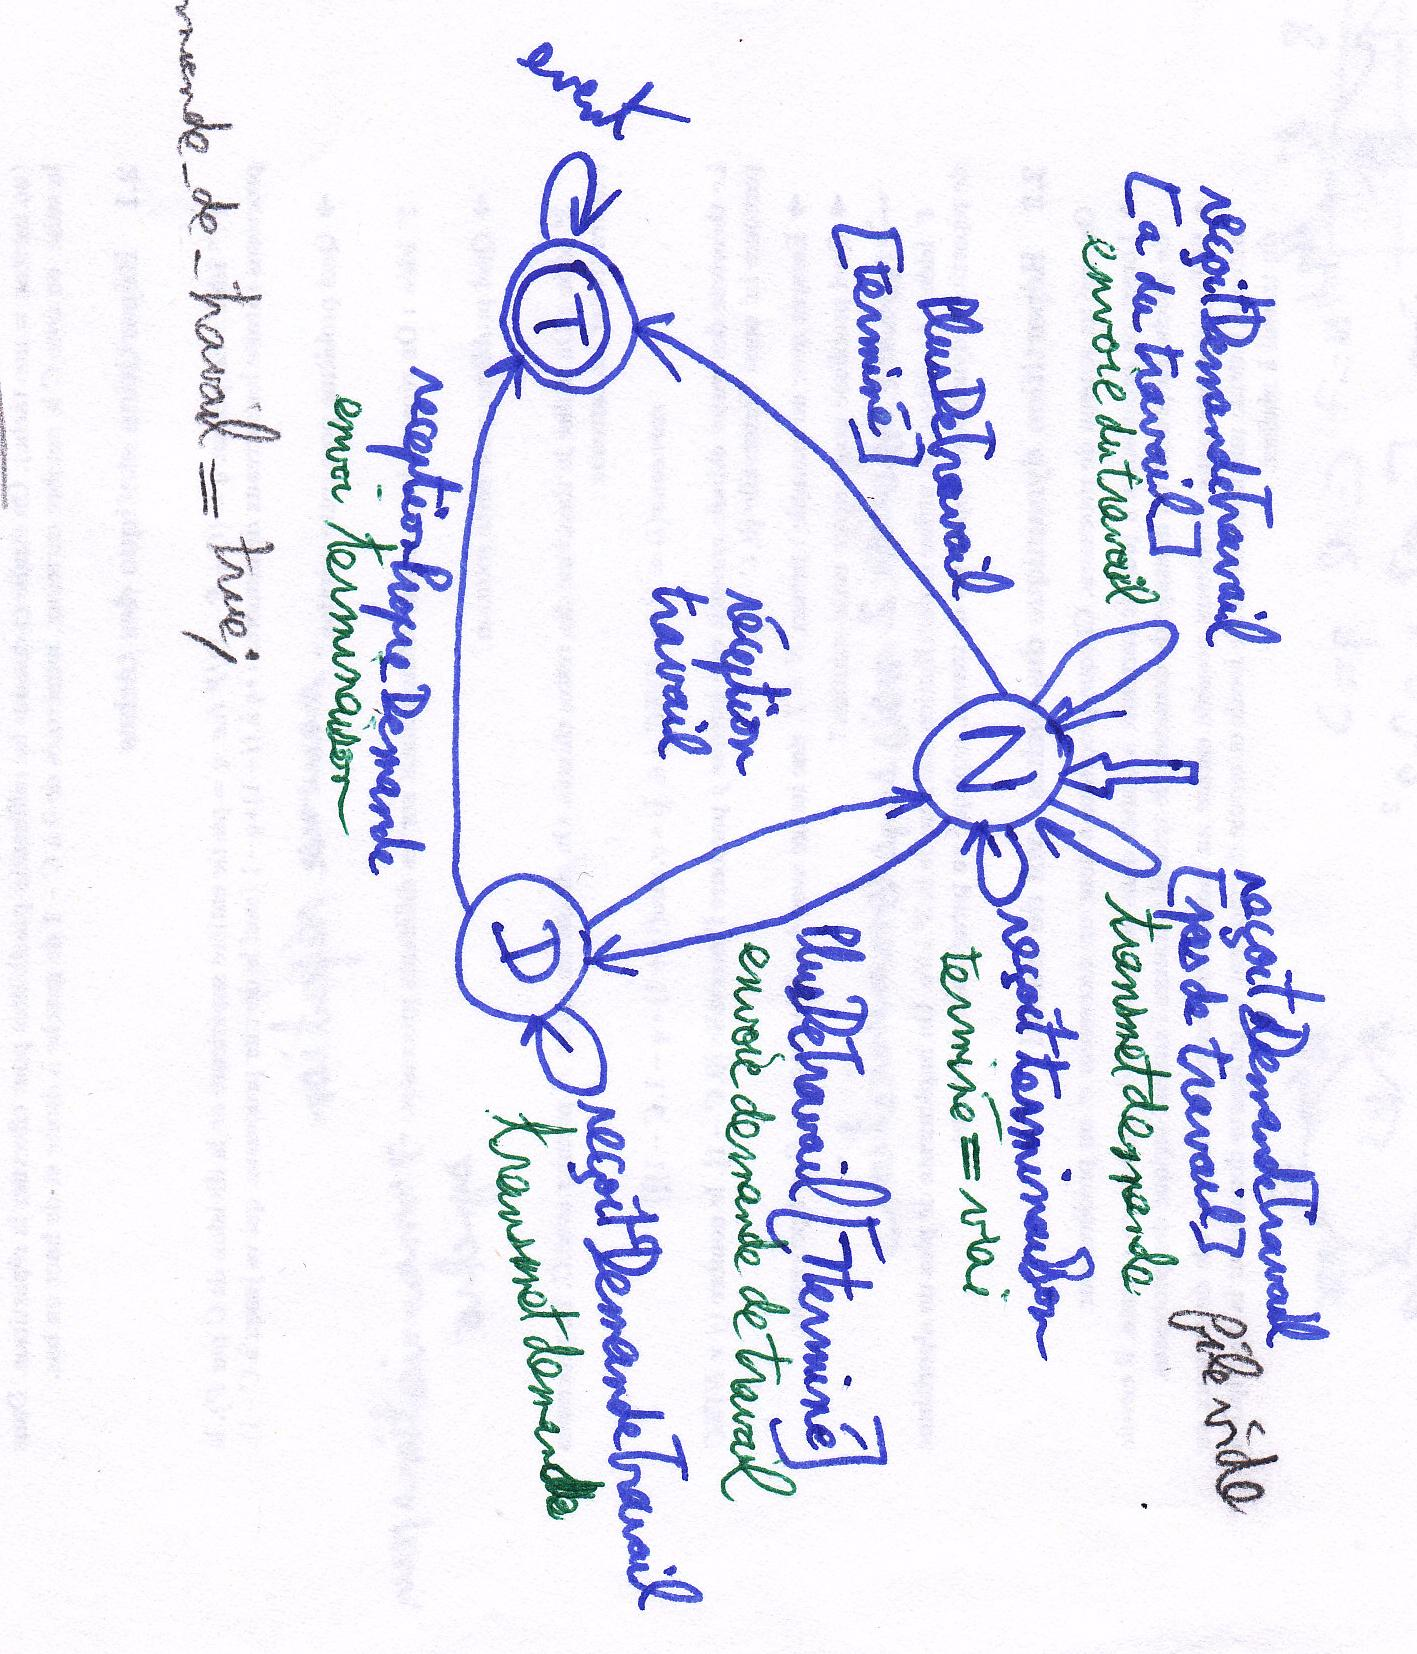
\includegraphics[width=0.6\textwidth]{automate.jpg}
\caption{Automate d'un processus secondaire pour les communications réseau}
\label{fig:diff}
\end{figure}

Afin de tester le bon fonctionnement de la transmission des taches, nous avons implémenté un système de taches factices permettant de créer des taches de longueur variable au lieu du calcul des tuiles. Le but est de créer un nombre différent de taches sur chaque processus et de vérifier que la charge de calcul est la même sur chaque processus.

% /section end

\section{Exécution \& tests} % (fold)
\label{sec:execution}

Pour ce projet, nous avons effectué des tests de validation sur quelques fonctions, afin de s'assurer que celles-ci marchaient correctement, et pouvoir plus facilement isoler les problèmes. 
De même, le code a été segmenté pour permettre une lecture plus aisée de l'ordre dans lequel s'effectuent les diverses opérations.

\section{Performances} % (fold)
\label{sec:perf}

Une série de tests est lancée sur différentes tailles de matrice plusieurs fois, afin d'obtenir des temps d'exécution moyens.
Les courbes de performances ont été tracées avec gnuplot et permettent de savoir où le programme passe le plus de temps (Fig. \ref{fig:diff}). On peut voir que pour des dimensions de matrice de plus en plus grandes, c'est surtout le calcul de la multiplication qui augmente. En effet, nous ne faisons pas varier le nombre de processus, tous les tests sont effectués avec quatre processus. On observe une augmentation linéaire du temps de calcul une fois que les processus ont suffisamment de calcul à effectuer.

%\begin{figure}[H]
%\centering
%\includegraphics[width=0.8\textwidth]{diff.png}
%\caption{Temps d'exécution des différentes parties du programme}
%\label{fig:diff}
%\end{figure}

Si l'on compare la figure précédente à la figure \ref{fig:sp}, la parallélisation s'améliore avec la taille du problème pour atteindre un pic juste en dessous de 4. Nous avons fait les comparaisons avec MKL sans parallélisation. Il faut cependant tenir compte du fait que MKL est déjà très optimisé, et nos communications ralentissent légèrement le programme rendant difficile d'atteindre un speed up de 4. On remarque également deux baisses de speed up sur la courbe. Ces baisses sont certainement dues à la taille des caches, et dans le deuxième cas pour les matrices de taille 4096*4096, à des accès à la mémoire RAM.

%\begin{figure}[H]
%\centering
%\includegraphics[width=0.8\textwidth]{Speedup.png}
%\caption{Accélération de notre programme par rapport au code séquentiel}
%\label{fig:sp}
%\end{figure}

% section \ (end)



\end{document}
